\section{User Control}
	
	Whilst the majority of this project is the physics, I think it is important that it is possible to interact with the simulation to be able to watch it more effectively. To this end I have built a command system which allows the user to control parts of the simulation along with certain key bindings.
	
	\begin{figure}[h]
		\begin{itemize}
			\item \textbf{+}/\textbf{-} $\rightarrow$ Speed up/slow down the simulation
			\item \textbf{LSHIFT} + \textbf{+}/\textbf{-} $\rightarrow$ Zoom in/out
			\item \textbf{LEFT}/\textbf{RIGHT} $\rightarrow$ Pan around the simulation horizontally
			\item \textbf{UP}/\textbf{DOWN} $\rightarrow$ Pan around the simulation vertically
		\end{itemize}
		\caption{Key bindings for the simulation}
		\label{fig:keybindings}
	\end{figure}
	
	\begin{figure}[h]
		\begin{itemize}
			\item track $<$particle num$>$ $\rightarrow$ Track a certain particle
			\item cleartrack $\rightarrow$ Clear the tracker, allow free movement
			\item show $\rightarrow$ Print a list of particles to STD Out
			\item forces $\rightarrow$ Toggle rendering of forces
			\item col $<$on/off$>$ $\rightarrow$ Render collision forces even if force rendering disabled
			\item particle $<$particle num$>$ $\rightarrow$ Centre view on a particle
			\item pause $\rightarrow$ Pause the simulation
			\item slow $\rightarrow$ Slow down the simulation to 10 UPS
			\item 1 $\rightarrow$ Set the maximum UPS to 1 (real time)
			\item speed $<$UPS$>$ $\rightarrow$ Set the speed of the simulation (sets max UPS)
			\item noCap $\rightarrow$ Set the max UPS to -1, effectively removing the cap on update speed
			\item scale $<$scale$>$ $\rightarrow$ Set the zoom so that one of the scale = 1 pixel (options: mm, cm, m, km)			
			\item zoom $<$zoom$>$ $\rightarrow$ Set the zoom to a specific number $zoom \in (0, \sim1.7\times10^{308})$
			\item pauseCollision $\rightarrow$ Pause the simulation on every collision
			\item exit $\rightarrow$ Exit the simulation
			\item run $<$simulation$>$ $\rightarrow$ run a specific simulation
			\item simulations $\rightarrow$ List the simulations available
			\item restart $\rightarrow$ Restart then current simulation
		\end{itemize}
		\caption{Commands for the simulation}
		\label{fig:commands}
	\end{figure}
	
	\begin{figure}
		\centering
		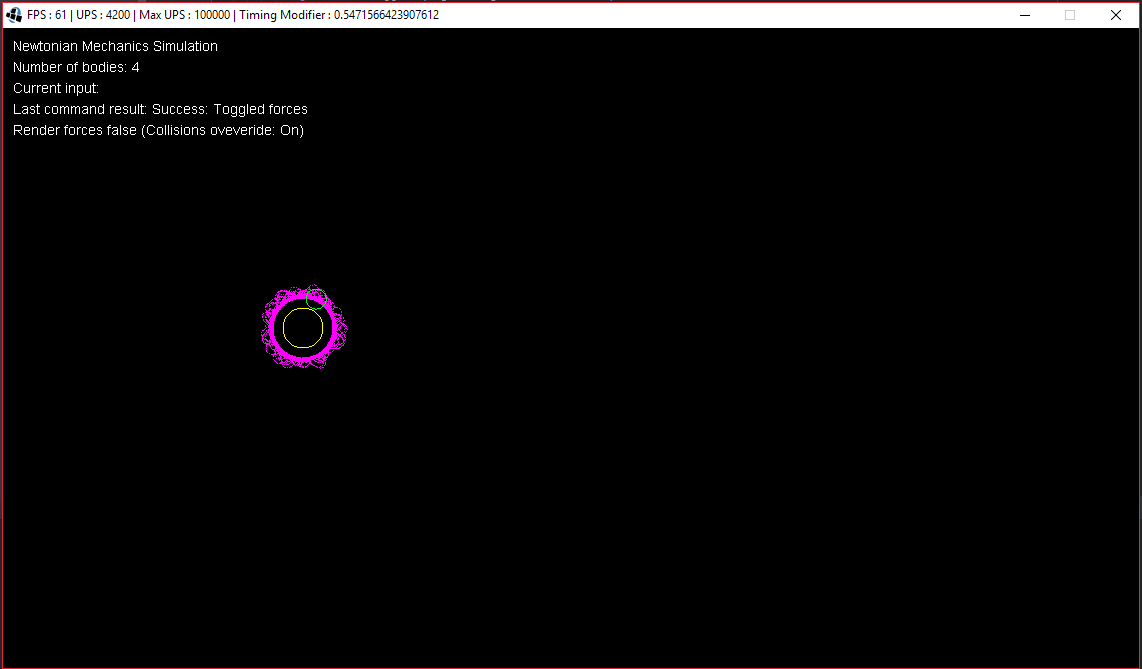
\includegraphics[width=\textwidth]{ux1}
		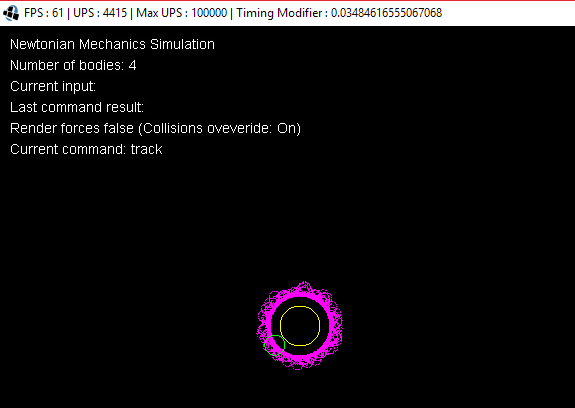
\includegraphics[width=\textwidth]{ux2}
		\caption{Information about the simulation displayed in the top left corner}
		\label{fig:uxImg1}
	\end{figure}

	I also implemented the ability for the user to track a specific particle over the course of the simulation and to export that data to excel in a .csv format. This allows the user to watch simulations where the scales are too big for the realtime graphics.
	
	